\section{Overview}
\setauthor{Lasinger Christoph}
The main focus of the project Animotion lies on the technical functionality 
of the translation of human face and body gestures captured by a camera to 
a VRM and the AI behind it. Therefore, the design of the website, on which
this functionality is displayed, mostly serves that focus. Besides the 
omepage, there are only four other webpages i.e., one showing the controlling 
of the model and the other three being minor ones, displaying less significant 
features.

\section{Homepage}
\setauthor{Lasinger Christoph}
As seen in figure \ref{fig:homepage} below, the homepage of the website starts with a big text
displaying the name of the project in a glitchy font with an even more glitchy
animation in order to immediately draw the user's attention. After that comes a
significantly smaller text in a less emphasizing colour, as it does not need to
be read by the user right away, simply giving instructions on what can be done
with the three images of 3D models below. As they stand in the centre of the page,
the three VRMs are on the first things one notices when visiting the website, which
is desired because clicking on one of them sends the user to the main page, where
the main functionality lies. Just for a pleasant effect, hovering over one of the
images displays a moving borderline, alternating between purple and pink. Below
each image is a button that navigates to another part of the website. Lastly, the
background for this page and the website in general is mostly black with one mirrored
girl on the side, mostly serving as nice accent and filling the rest of the page.
The main colour used for most design elements, be it the navigation buttons, main
fonts, back buttons, and so on is a nice-looking shade of purple (hex colour code 8d4be0 to be exact). 
Less significant text, for example that of the bottom navigation
buttons, is simply white and any other text that is of moderate importance is mixture
between the two, created by taking the average of both colour values.

\\
\begin{figure}[htb]
    \centering
    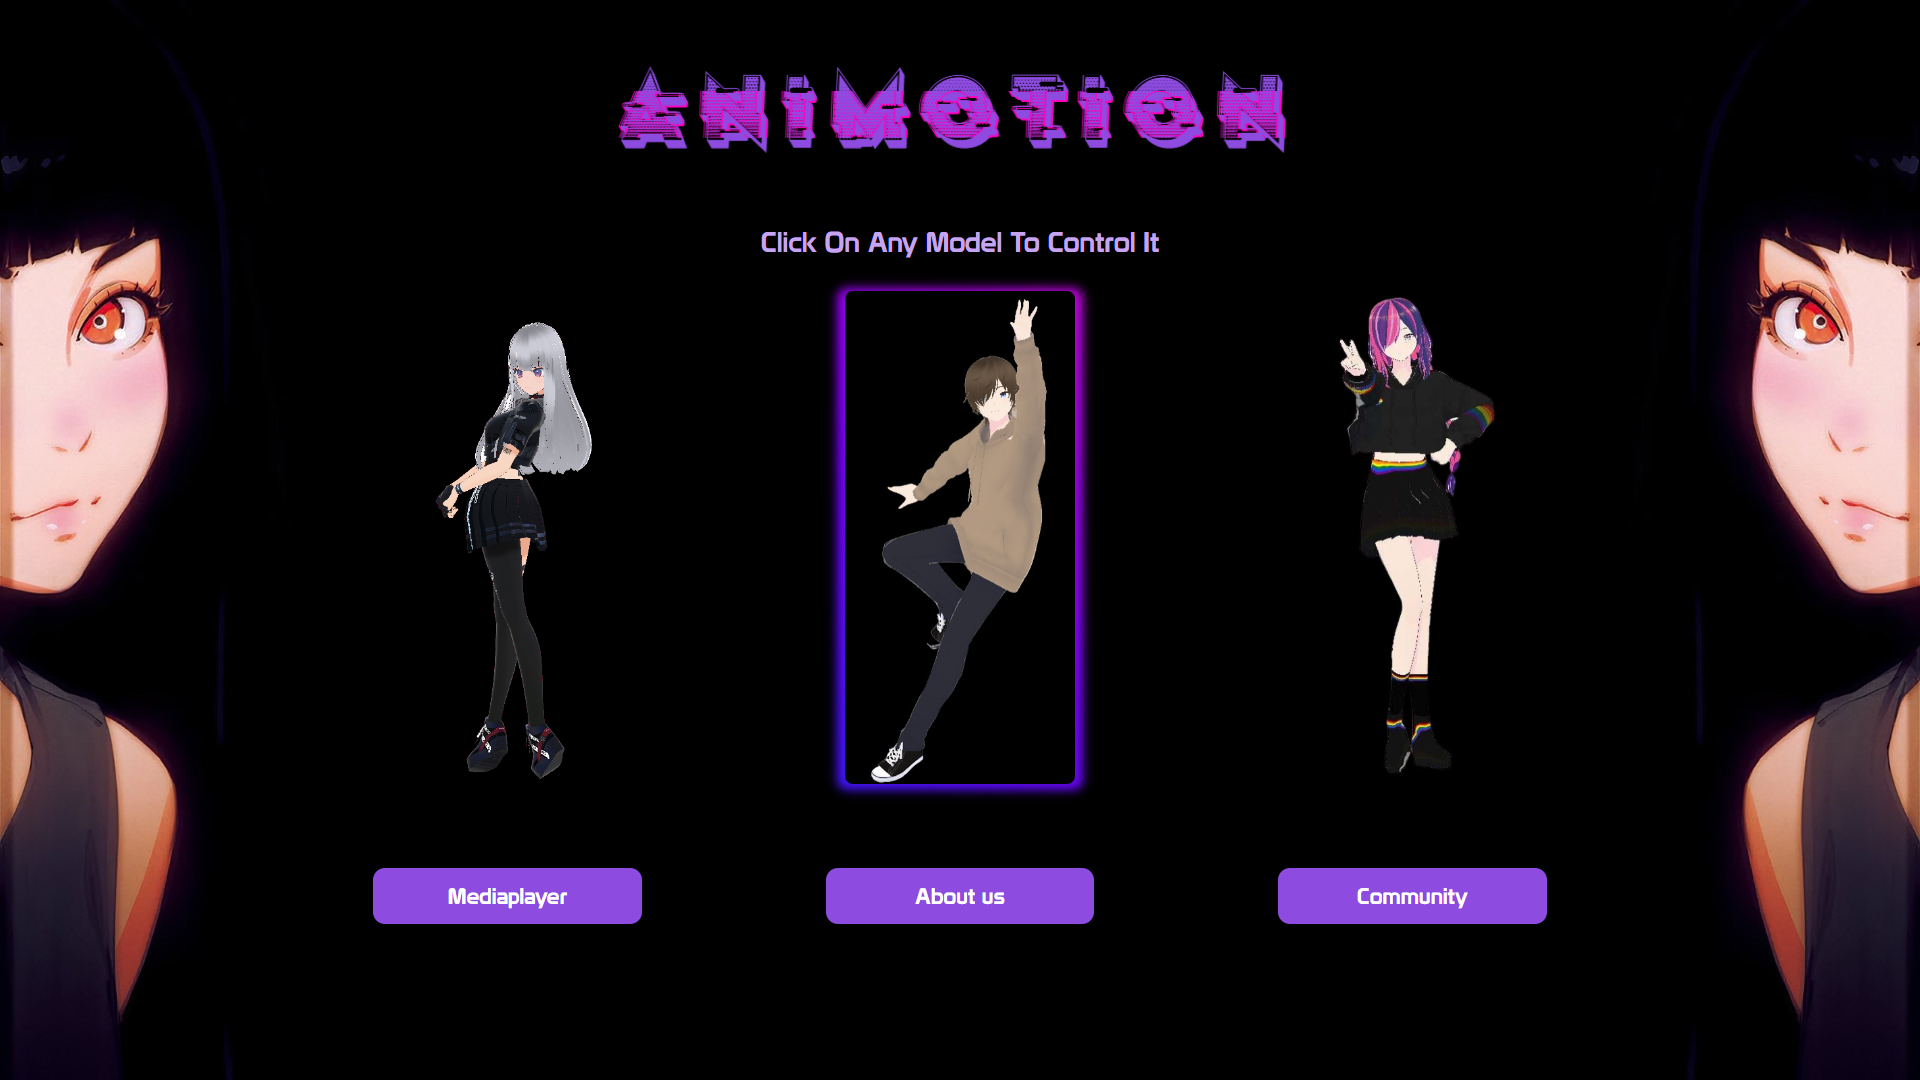
\includegraphics[width=0.8\textwidth]{pics/Animotion_homepage.png}
    \caption{Homepage of the website}
    \label{fig:homepage}
\end{figure}
\\

\section{Main page}
\setauthor{Lasinger Christoph}
After hovering over and eventually left clicking one image of the models on the homepage,
the user lands on the following page, shown in figure \ref{fig:mainpage} below. While the user takes in
the content of the page, the website quickly loads the model in the background. After it
finishes loading, it is displayed on the screen and the camera starts taking in information
and relaying it to the AI, which takes a short while. Once that process is done, an image
of the AI recognizes is laid over the camera window and the VRM starts moving according
to face and body gestures done by the user. In case the user wants to see a different, or
bigger part of the model, the controls are shown in the top right corner. The recording
feature and the controls to it can be found in the bottom left corner, where the user can
start or stop recording what is displayed on the website any time. Lastly, in the top left
corner is a button that removes any UI elements, that can in some situations be an unnecessary,
leaving the user to fully focus on the moving model and button that leads back to the homepage
to for example choose a different model. Because of the UI elements lingering in each corner,
the general background did simply not look good on this specific page and a different background,
that does not particularly draw any attention to it, was chosen.

\\
\begin{figure}[htb]
    \centering
    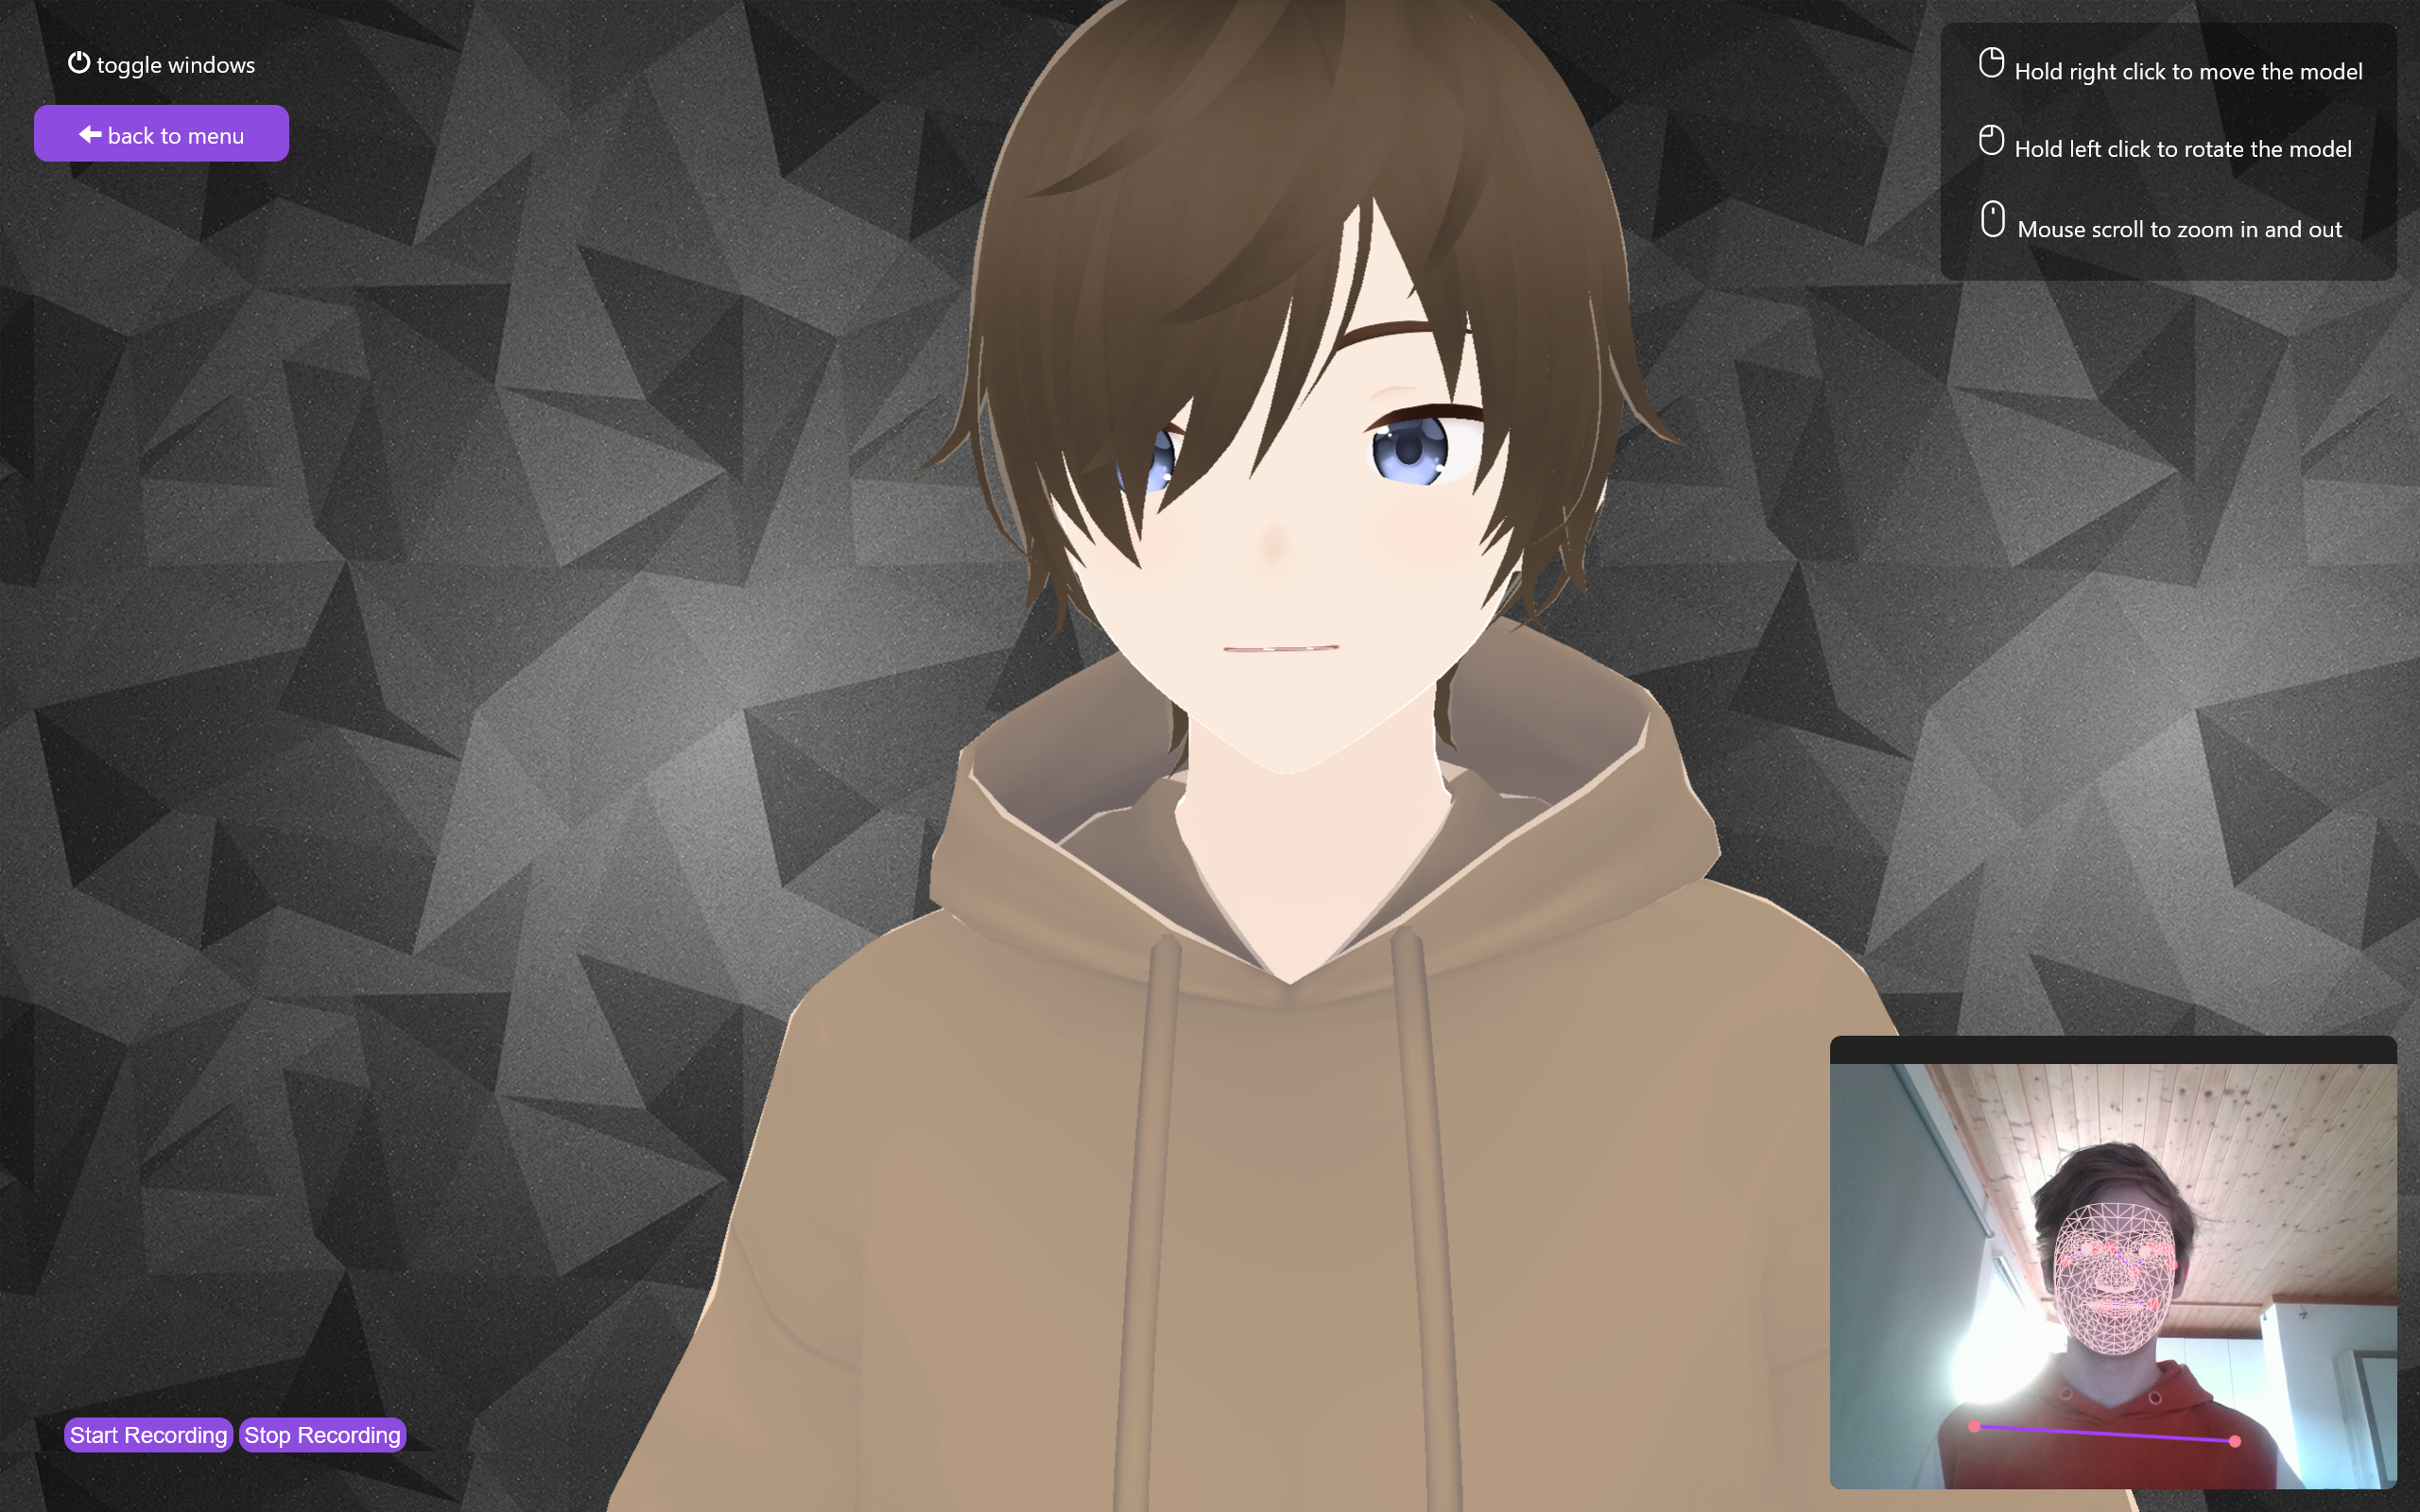
\includegraphics[width=0.8\textwidth]{pics/Animotion_mainpage.png}
    \caption{Main page of the website}
    \label{fig:mainpage}
\end{figure}
\\

\section{Community page}
\setauthor{Lasinger Christoph}
On the community page a discord server specifically created for Animotion is presented along with
general information about said community. This community was envisioned to be a place for people
to share music and dance videos created by recording a chosen VRM following a person's recorded
movements on the main page with each other. Additionally, any questions regarding the project could
be answered and required assistance could be provided.

The discord server is shown on the web page by embedding a widget through a HTML element named
iframe, a combination of the words inline and frame that essentially renders code taken from a
referenced source as if it was a separate website and places it within the parent page. An iframe
can independently loaded its own CSS and JavaScript and asynchronously refreshed and reloaded as
well. As an ordinary HTML element, it is possible to customize iframes by setting its properties,
such as position, size, source, security context, border, etc. It is recommended to avoid excessive
usage of them, as they require significant amounts of memory and processing power and can thusly
negatively impact a website's performance. %source [19]

The widget on this community page displays what members of the server are currently online and the
voice channel they reside in, which can be valuable information to someone who might decide to join
possible conversations depending on who is participating in them.

The specific iframe and its set properties can be seen in following code snippet shown in listing \ref{lst:iframe}.

\begin{lstlisting}[language=Python,caption=iframe used for discord widget,label=lst:iframe]
    <iframe className="discord-iframe" src="https://discord.com/widget?id=1035647726634934382&theme=dark"
    allowtransparency="true" frameBorder="0" sandbox="allow-popups allow-popups-to-escape-sandbox allow-same-origin allow-scripts"></iframe>
\end{lstlisting}
The usage of said iframe results in the following web page as seen in figure \ref{fig:communitypage}.

\\
\begin{figure}[htb]
    \centering
    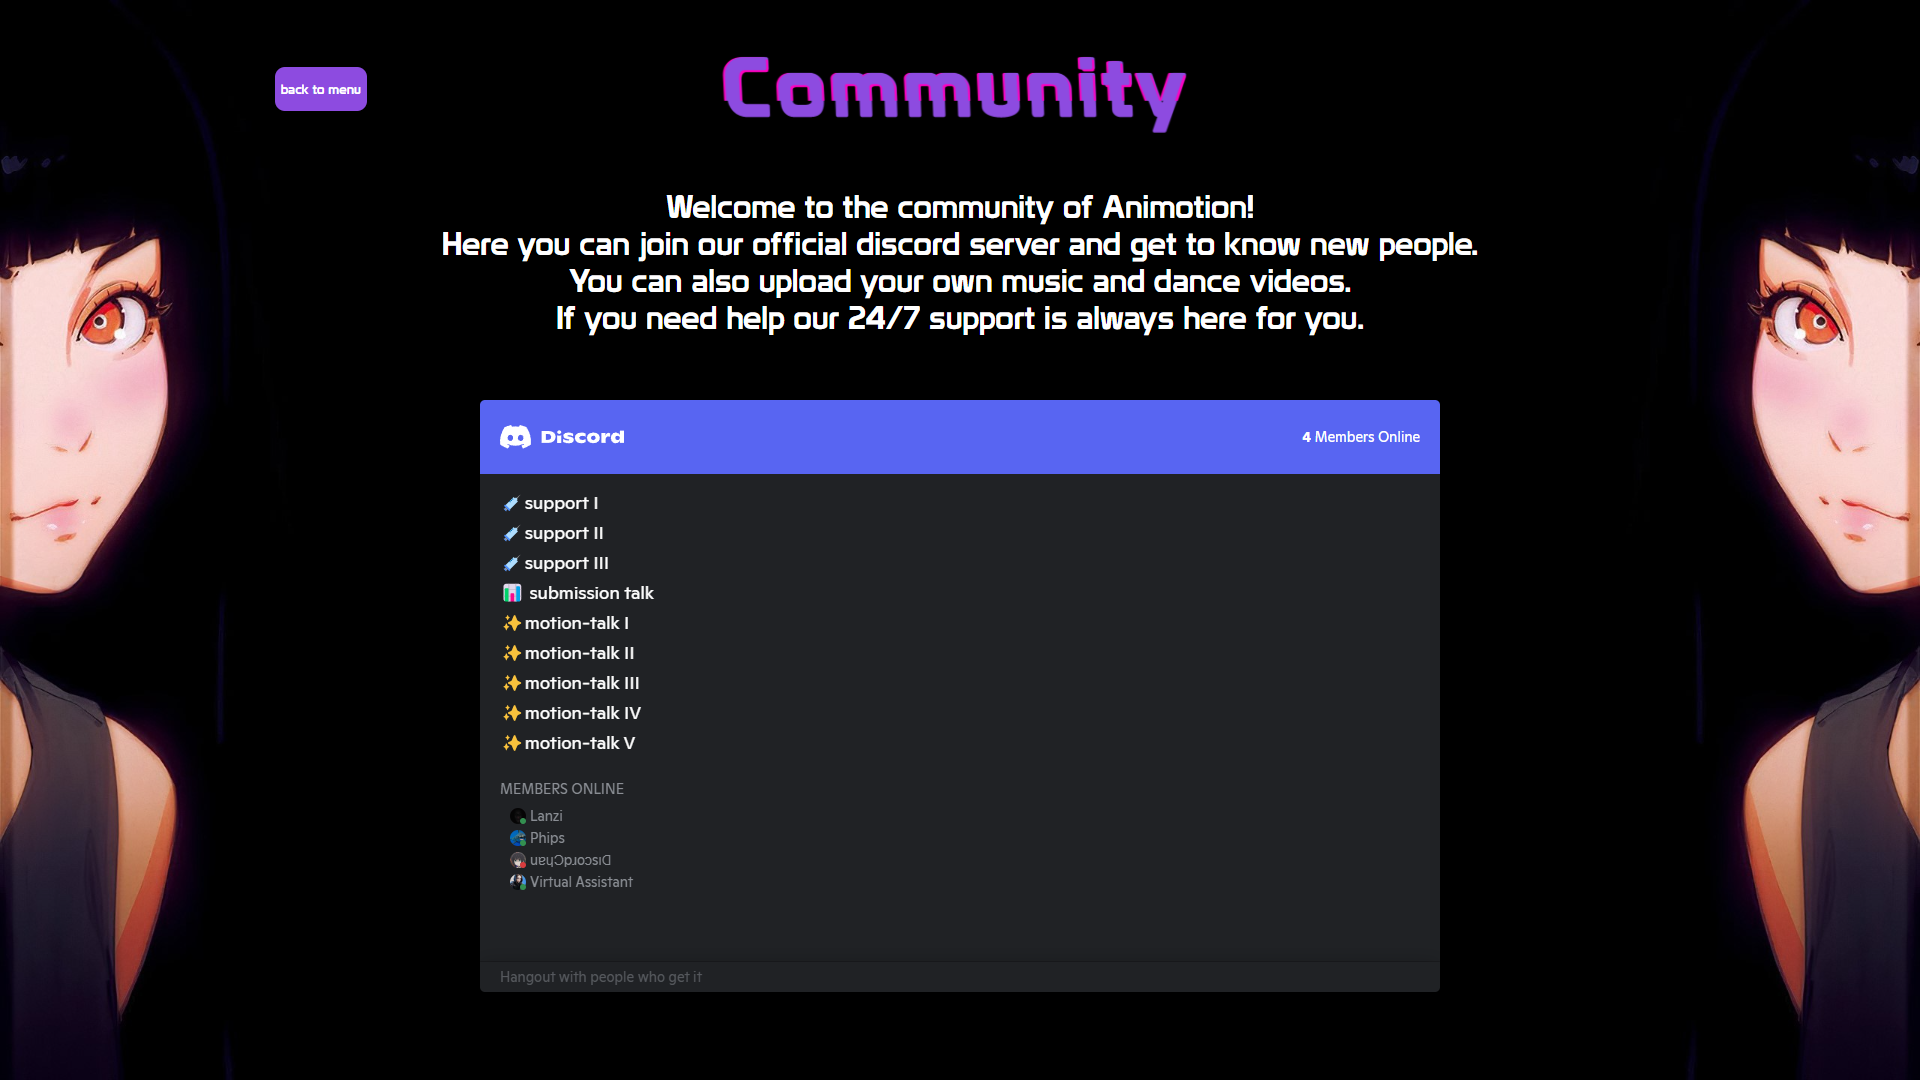
\includegraphics[width=0.8\textwidth]{pics/Animotion_community.png}
    \caption{Main page of the website}
    \label{fig:communitypage}
\end{figure}
\\

\section{About us page}
\setauthor{Lasinger Christoph}
The centre button of the homepage leads to the about-us-page, derived from the commonly seen about-me-page
made by individual developers and adapted to the fact that Animotion was created by a two-person team. While
it does not contain particularly important information, it presents a bare minimum amount of information
about us, the developers of this project.

Additionally, in order to always be legally covered in case Animotion evolves into a larger project in the
future a legal disclosure can be found on this page as well. It informs the reader of our real names and an
address, email, and phone number to reach out to.

\section{Mediaplayer page}
\setauthor{Lasinger Christoph}
Lastly, there is the media player page where embedded YouTube videos of VRMs dancing to certain songs are displayed.

